\documentclass[20pt,margin=1in,innermargin=-4.5in,blockverticalspace=-0.25in]{tikzposter}
\geometry{paperwidth=42in,paperheight=30in}
\usepackage[utf8]{inputenc}
\usepackage{amsmath}
\usepackage{amsfonts}
\usepackage{amsthm}
\usepackage{amssymb}
\usepackage{mathrsfs}
\usepackage{graphicx}
\usepackage{adjustbox}
\usepackage{enumitem}
\usepackage[backend=biber,style=numeric]{biblatex}
\usepackage{emory-theme}
\usepackage[scaled]{helvet}
\usepackage[T1]{fontenc}
\usepackage{tikz}
\usepackage{wrapfig}
\usetikzlibrary{shapes.geometric,calc}


\usepackage{mwe} % for placeholder images

\addbibresource{refs.bib}

% set theme parameters
\tikzposterlatexaffectionproofoff
\usetheme{EmoryTheme}
\usecolorstyle{EmoryStyle}

\title{Parallelization in Multiple Imputation}
\author{Sven Nekula, Joshua Simon and Eva Wolf}
\institute{Otto Friedrich University, Bamberg}
\titlegraphic{
\includegraphics[width=0.06\textwidth]{img/uni_ba_logo_100_blau.png}}

\newcommand\score[2]{%
	\pgfmathsetmacro\pgfxa{#1 + 1}%
	\tikzstyle{scorestars}=[star, star points=5, star point ratio=5, draw, inner sep=1.3pt, anchor=outer point 3]%
	\begin{tikzpicture}[baseline]
		\foreach \i in {1, ..., #2} {
			\pgfmathparse{\i<=#1 ? "yellow" : "gray"}
			\edef\starcolor{\pgfmathresult}
			\draw (\i*1.75ex, 0) node[name=star\i, scorestars, fill=\starcolor]  {};
		}
	\end{tikzpicture}%
}

% begin document
\renewcommand\familydefault{\sfdefault}
\begin{document}
\maketitle
\centering
\begin{columns}
    \column{0.32}
    \block{What is Parallelization?}{
    	\begin{wrapfigure}{l}{7cm}
    		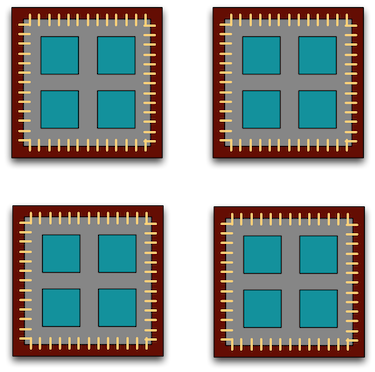
\includegraphics[width=7cm]{img/cpu.png}
    	\end{wrapfigure}
         Parallelization is a technique to fasten time-consuming computations. It uses all the cores on a CPU (Central Processing Unit) parallely and splits up the computational work on them. Afterwords, the results are merged. This can reduce the time needed for a task. \\
         \\
         \\
        
    }
	\block{Theory}{
		\textbf{Parallel Computing}\\
		\begin{wrapfigure}{r}{8cm}
			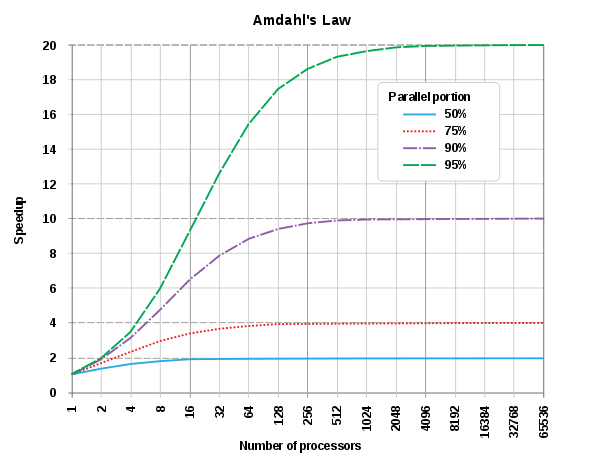
\includegraphics[width=8cm]{img/600px-AmdahlsLaw.svg}
		\end{wrapfigure}
		In parallel programming, the multiple cores of a computational system want to be used best to decrease computation time. Gene \textbf{Amdahl} was the first one to desribe the boundaries of that project: Every parallel process also requires additional workload, so called "data management housekeeping". The speed up through parallel processing will tend to 0 at a certain amount of processing units involved, as this \textbf{overhead} workload exceeds the capacity of the computational unit which it is assigned to.\\
		\textbf{Multiple Imputation}\\
		Multiple imputation is a method to complete a dataset with missing information. It relies on the estimation of the missing values through different methods. What is common to them is that we use not a single imputation run, but several. The results of all imputation runs are then merged and lead to realistic uncertainty of the estimators given the missing data. 
	}
	\block{Methodology}{
	\textbf{data generation} We used a simple data generator of normally distributed random variables. The data set created contains 10 variables, of which some depend on each other. The sample size created was n 10000. Expermients were compared to euqal settings with real data, and the results did not change the direction of the results. More complex data favor the mechanism of parallelization.\\
	\textbf{time measurement} was done with the \textit{system.time} function, which returns 3 values: User CPU-, User System- and Elapsed time. User CPU is the time needed by the current task such as an execution in R. System CPU describes the time needed by the operating system to organize that task such as opening folders or asking for the System time. Elapsed time is the Wall Clock time that passed while the function was running.\\
	\textbf{mice method} The method of the mice algorithm was set on defaut, pmm.\\
	\textbf{speed up}The speed\_up value is calculated by the serial time (runtime without parallelization) divided by the runtime of the current parallelization implementation \cite{cite:chapple2016mastering}. Values below one show that the parallelized run took longer than the serial run.\\
	}
    \column{0.36}
    \block{Results}{
        
        \vspace{1em}
        \begin{tikzfigure}[Runtime and Speedup from 1 up to 8 cores]
            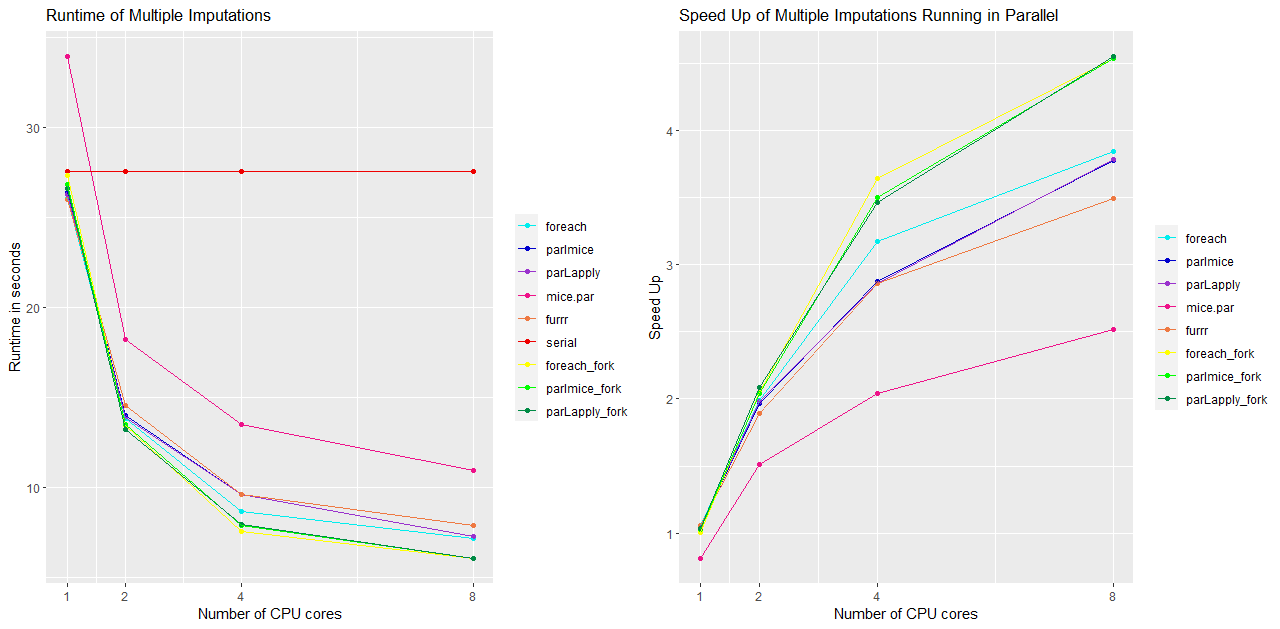
\includegraphics[width=1\linewidth]{img/runtime_ncores_speedup}
        \end{tikzfigure}
        \vspace{1em}
       
       \vspace{1em}
       \begin{tikzfigure}[Runtime and Speedup from 1 up to 8 cores]
       	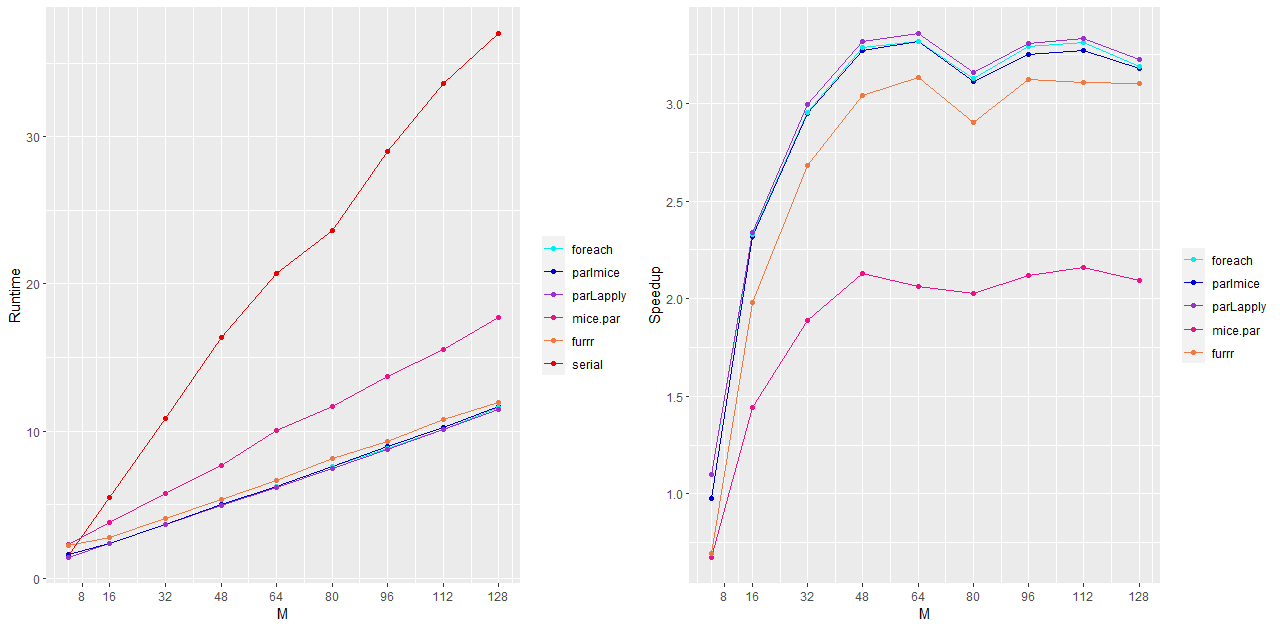
\includegraphics[width=1\linewidth]{img/runtime_nimp_speedup_resized}
       \end{tikzfigure}
       \vspace{1em}
       
      \vspace{1em}
      \begin{tikzfigure}[Runtime and Speedup from 1 up to 8 cores]
      	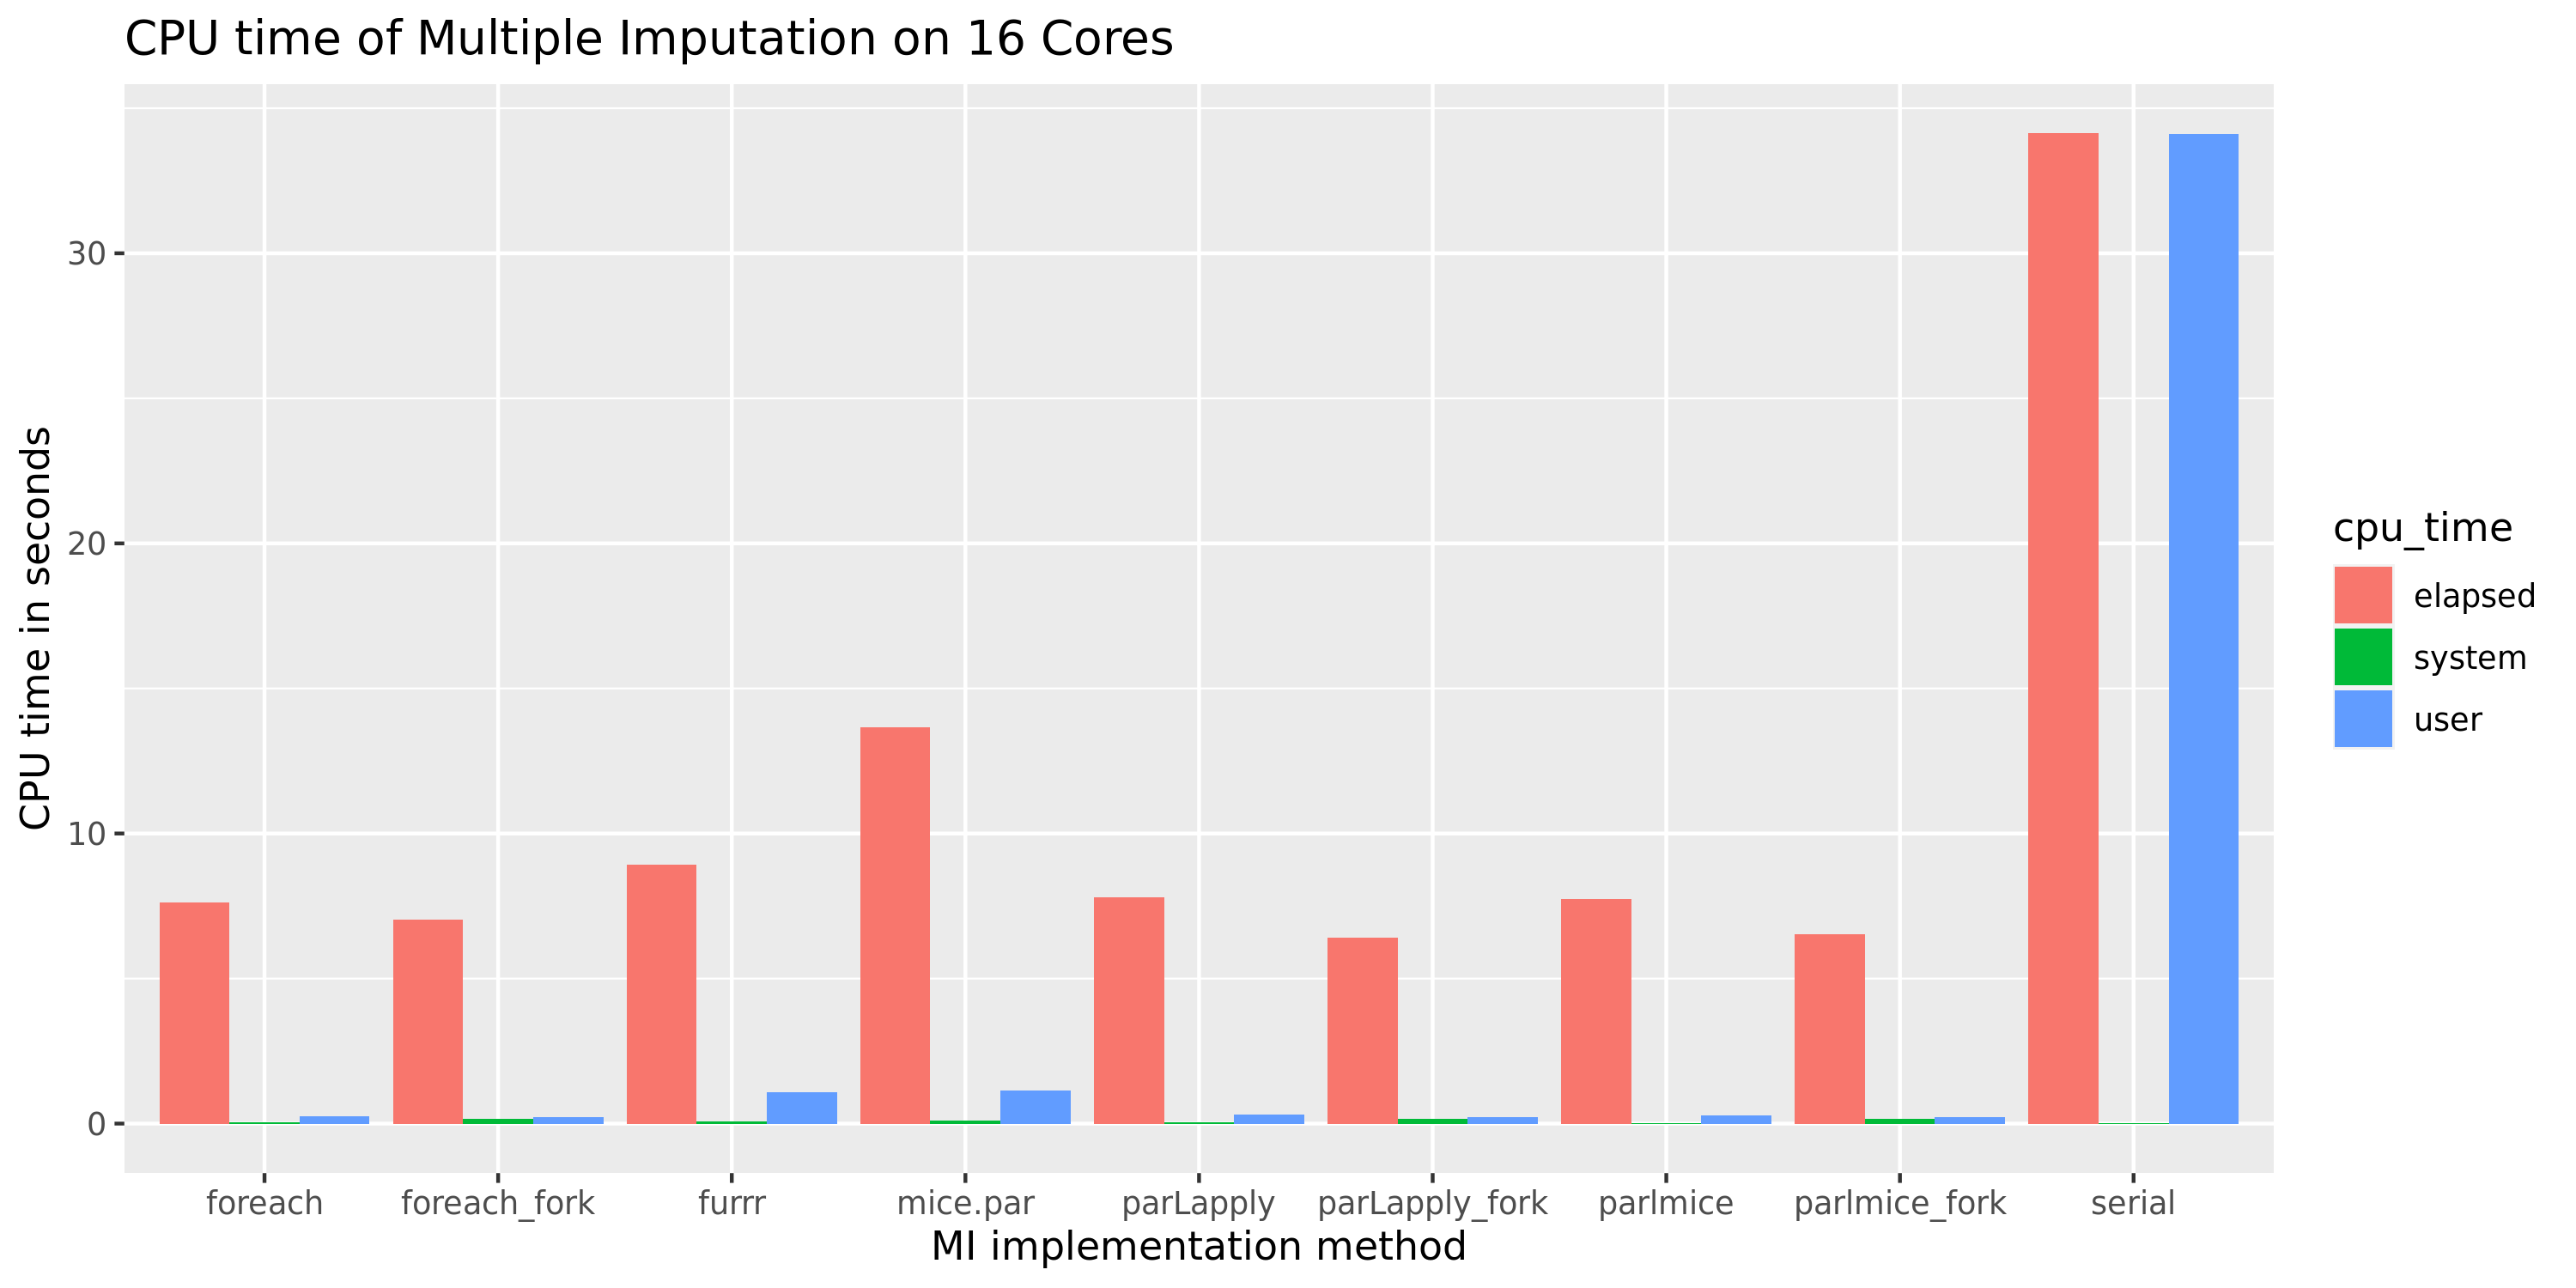
\includegraphics[width=0.7\linewidth]{img/2022-01-15_benchmark_core_Linux_cpu_time}
      \end{tikzfigure}
      \vspace{1em} 
    }

    \column{0.32}
    \block{Comparison of Implementations}{
    	
    	\textbf{foreach::foreach} usability \hspace{-1mm}\small{\score{2.4}{5}} \hspace{1cm} runtime\hspace{-1mm}\small{\score{2.4}{5}}\\
    	\\
    	\textbf{mice::parlmice} usability
    	\hspace{-1mm}\small{\score{2.4}{5}}\\
    	\\
    	\textbf{micemd::mice.par} usability
    	\hspace{-1mm}\small{\score{2.4}{5}}\\
    	\\
    	\textbf{parallel::parLapply} usability
    	\hspace{-1mm}\small{\score{2.4}{5}}\\
    	\\
    	\textbf{purrr::future\_map} usability
    	\hspace{-1mm}\small{\score{2.4}{5}}\\ 
    	\\
    }
    \block{Application}{
    \begin{wrapfigure}{r}{6cm}
    	
\includegraphics[width=5cm]{img/disk.framing}
    \end{wrapfigure}
	For \textbf{disk framing}, parallelization is a useful tool	to decrease computation time. Disk framing seperated larger-than-RAM datsets into several chunks of data, which are then treated seperately for the task to perform. Afterwords, results are merged again. With the help of parallelization, chunks of data can be processed parallely and so calculation time is reduced.\\
	
}
    \block{References}{
        \vspace{-1em}
        \begin{footnotesize}
        
        \printbibliography
        
        \end{footnotesize}
    }
\end{columns}
\end{document}